\chapter{Ergebnisse}


- Auswertung (Qualitative Auswertung)\\
- Lauferkennung \\
- Rechenzeit: kein wesentlicher Unterschied (55 Sec und 57 Sec)

\section{Verifikationsversuche}

- Alle geplanten Szenarien wurden mind. einmal getestet.\\

- Die erste sowie letzte Szenarien wurden jeweils zweimal getestet.\\

Nach der Durchführung der Verifikationsveruchen werden die Ergebnisse analysiert und diskutiert. Die Lauferkennung ist ein großer Teil dieser Arbeit und wird demnächst mit den tatsächlichen Daten sowie die integrierte Aktivitätserkennungsfunktion verglichen.
\section{Lauferkennung}
In der \autoref{fig:Speed_Groundtruth_MotionClass_GoogleMD_Compare} werden die verschiedenen Methoden der Aktivitätserkennung sowie die Geschwindigkeit (oberste Grafik) dargestellt.

Die zweite Grafik zeigt die tatsächlichen Aktivitätsdaten (GroundTruth) und die Dritte zeigt die Ausgabe der im Rahmen dieser Arbeit implementierten Lauferkennung.
Die letzte Grafik stellt die Ausgabe der im Smartphone integrierten Aktivitätserkennung dar. Diese drei Grafiken unterscheiden zwischen drei Klassen:

**** Die Liste der Klassen als Tabelle hinzufügen. *****

\begin{figure}[H]
	\centering
	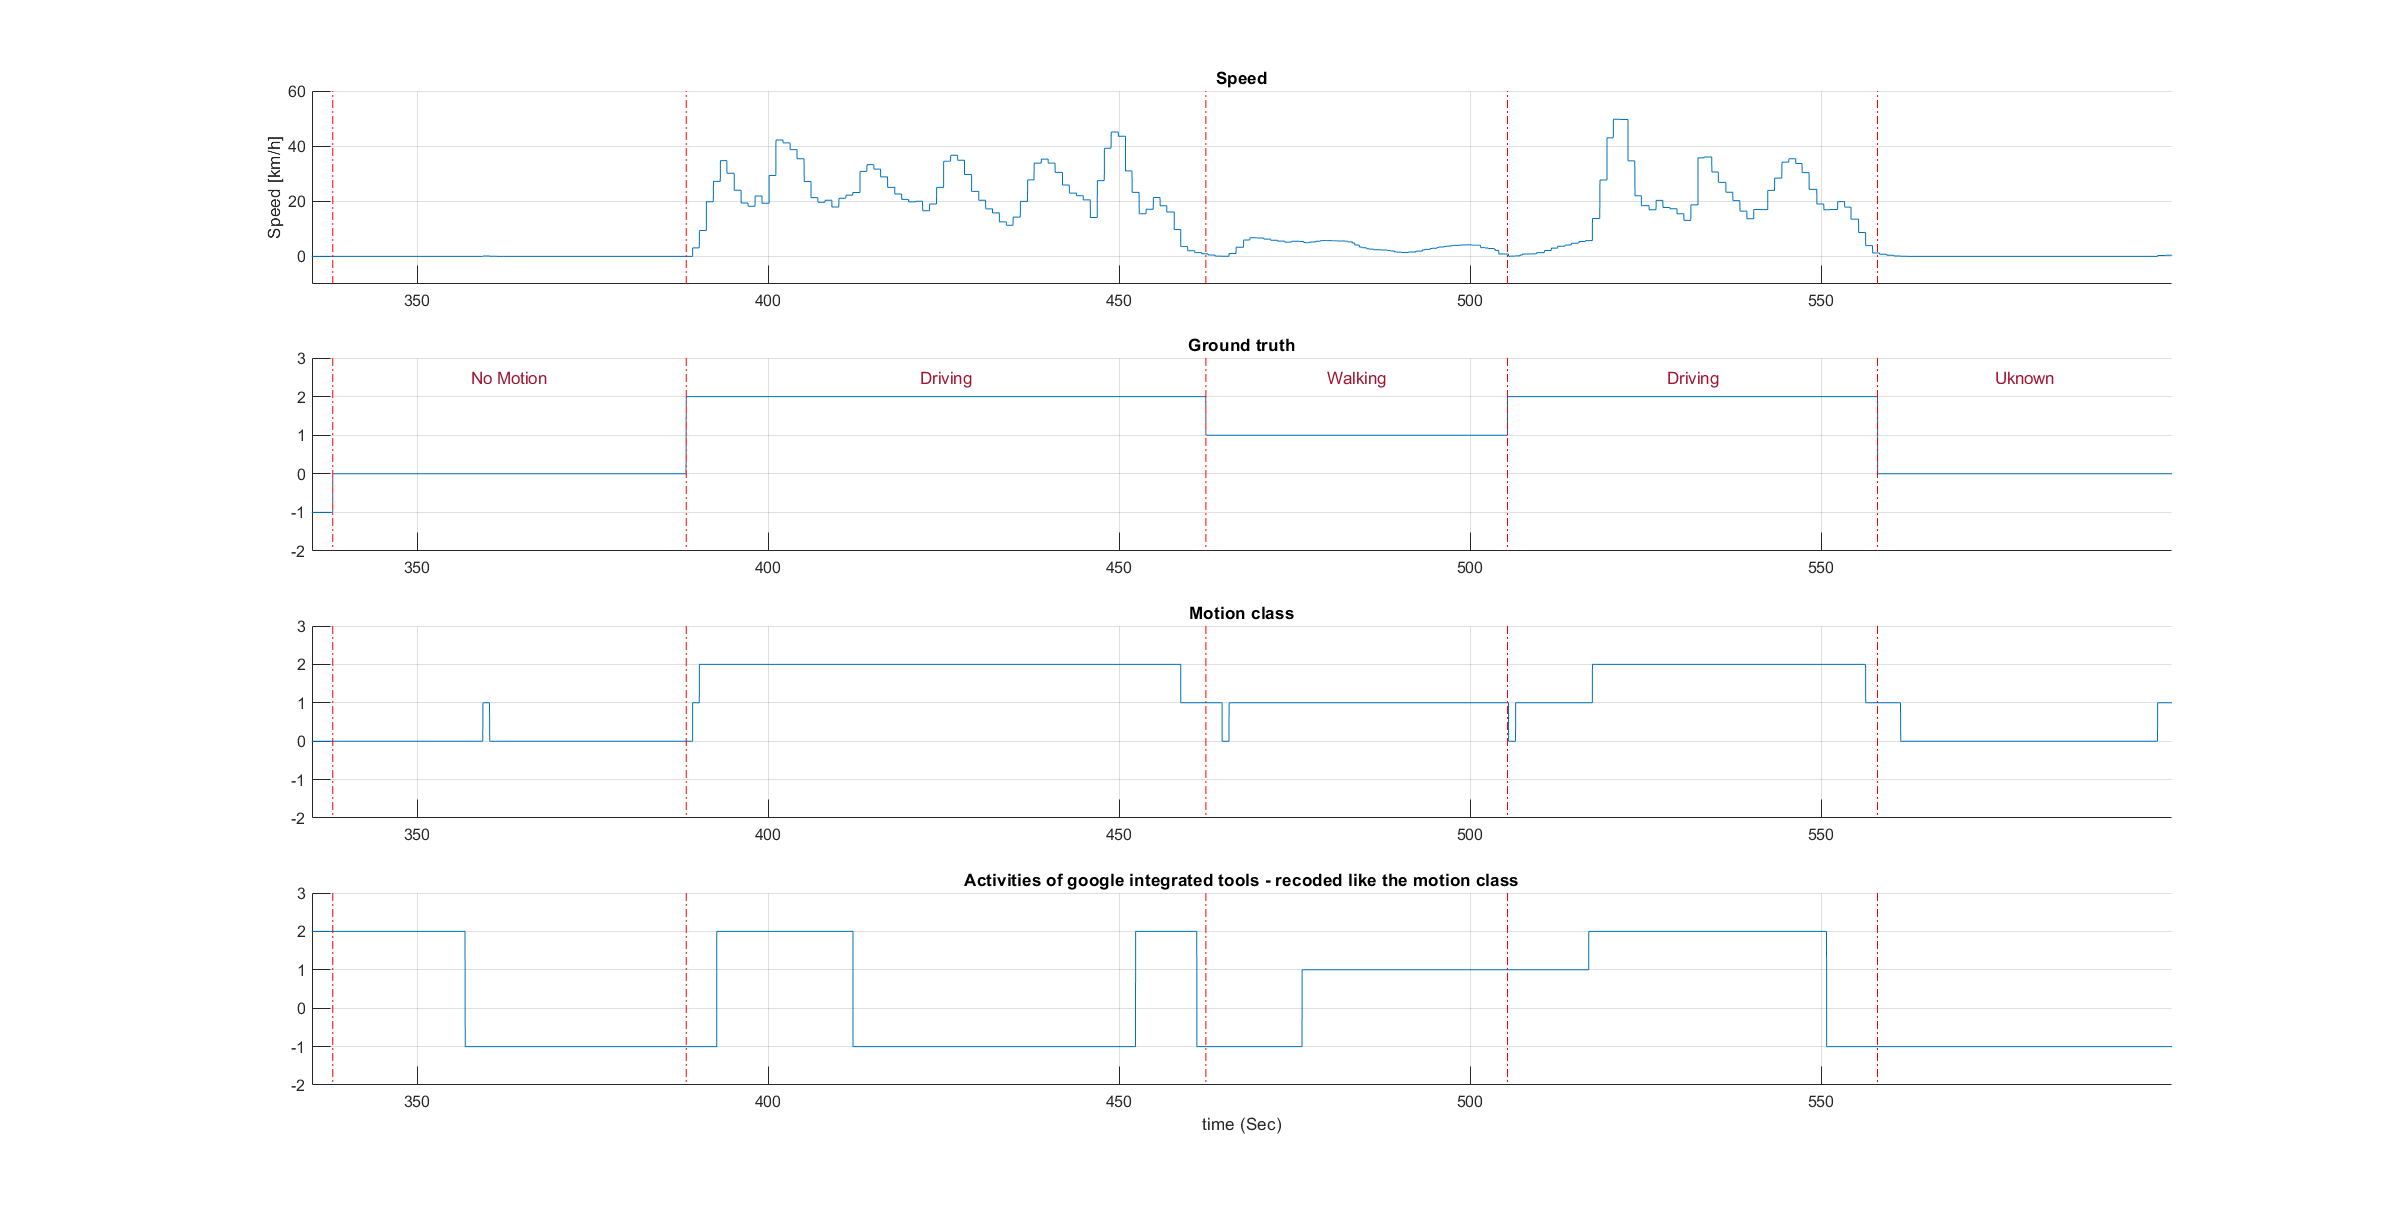
\includegraphics[width=\linewidth]{Bilder/Speed_Groundtruth_MotionClass_GoogleMD_Compare.png}
	\caption{Ergebnis des Lauferkkennungsmodells}
	\label{fig:Speed_Groundtruth_MotionClass_GoogleMD_Compare}
\end{figure}

Aus der Grafiken ist zu bemerken, dass die Klassifizierung durch das implementierte Modell sehr gute Ergebnisse liefert, die mit der Wahrheit mehr als $85\%$ übereinstimmt. Im Vergleich zu der Google-Aktivitätserkennung hat das Modell eine wesentlich bessere Aussage getroffen.



\section{Verschiedene Fahrerpositionierung}
Die \autoref{fig:Speed_Groundtruth_MotionClass_GoogleMD_Compare} zeigt vier verschiedene Grafiken mit der gleichen x-Achse (Zeit [Sec]).
In der ersten Grafik ist die Geschwindigkeit (blau) sowie die Alarmauslösung (lila) über die Zeit abgebildet.
Die zweite Grafik stellt die tatsächliche Daten der Fahrerposition (Sitzen, Stehen oder unbekannt) über die Zeit dar.
In der dritten Grafik ist der tatsächliche Verlauf Fahreraktivität (Fahren, Laufen oder unbekannt) dargestellt.
Die Kurve aus der letzten Grafik zeigt den Verlauf des Gerätswinkels im Vergleich zur ursprünglichen Platzierung während der Kalibrierung. 

\begin{figure}[H]
	\centering
	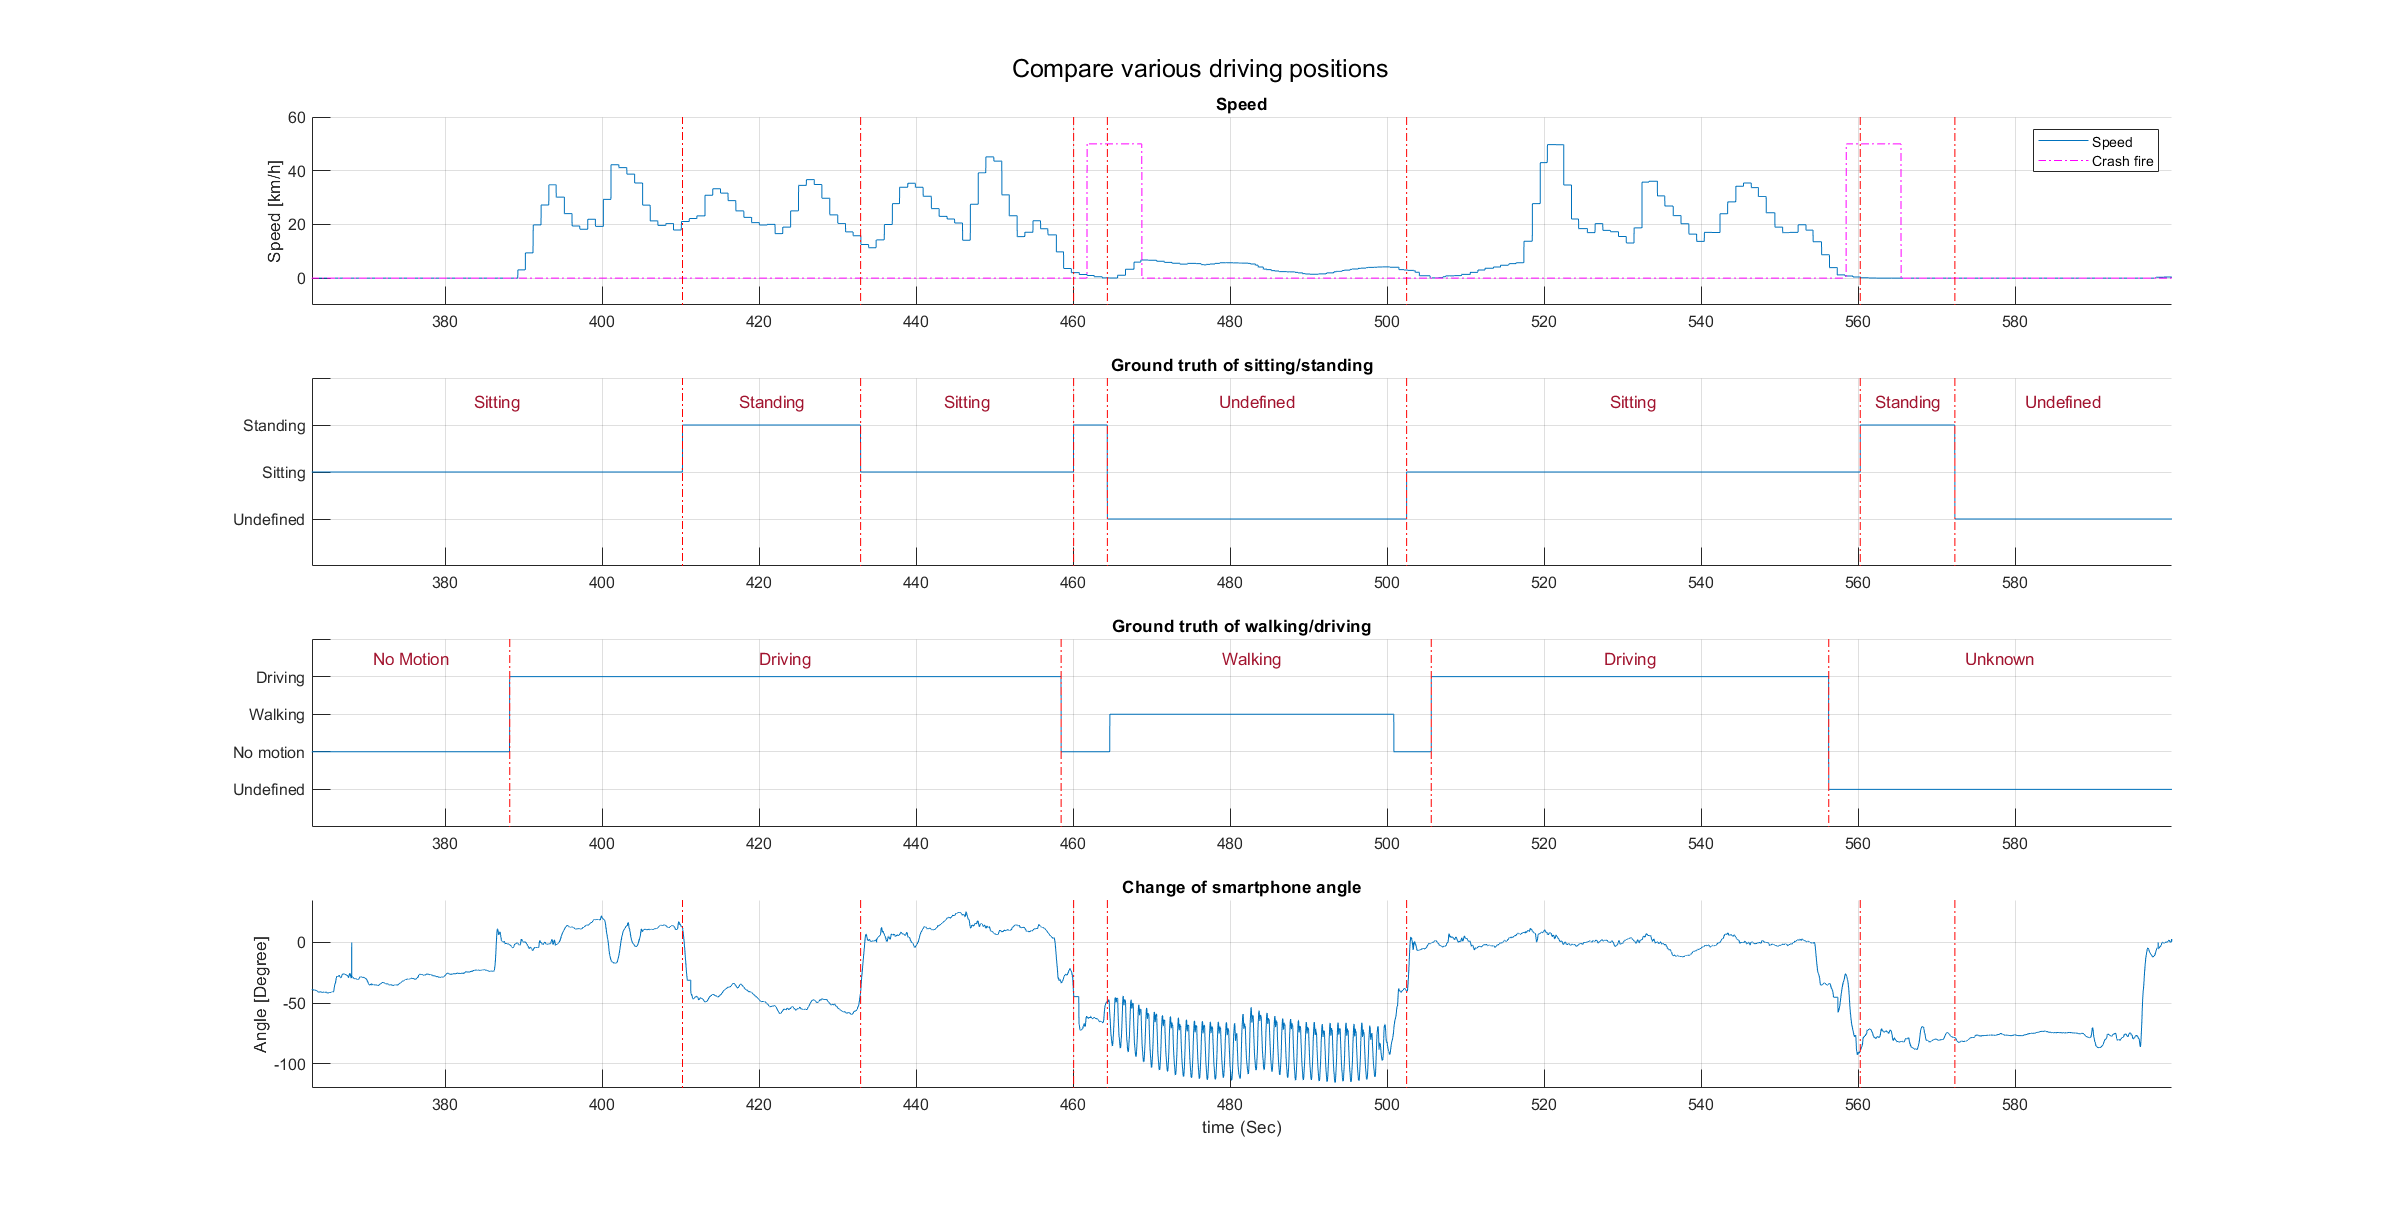
\includegraphics[width=\linewidth]{Bilder/Speed_Groundtruth_WalkStand_Compare.png}
	\caption{Vergleich der Fahrt in vertikaler und normaler Position}
	\label{fig:Speed_Groundtruth_WalkStand_Compare}
\end{figure}


Aus der \autoref{fig:Speed_Groundtruth_MotionClass_GoogleMD_Compare} ist Folgendes zu verstehen:

\begin{itemize}
	\item In der Zeitbereich zwischen $388 - 458$ s findet eine Fahrt statt, während dieser die Fahrerposition sich verändert hat. Der Fahrer ist für ca. $10$ s gestanden und wieder gesessen.
	\item In der Zeitbereich zwischen $465 - 505$ s ist die Versuchsperson gelaufen, deswegen lautet die Klassifizierung in der zweiten Grafik '"Unbekannt"', da die gedachte Klassen so ein Fall nicht abdecken.
	\item  
\end{itemize}

\section{Anhalten}

\begin{figure}[H]
	\centering
	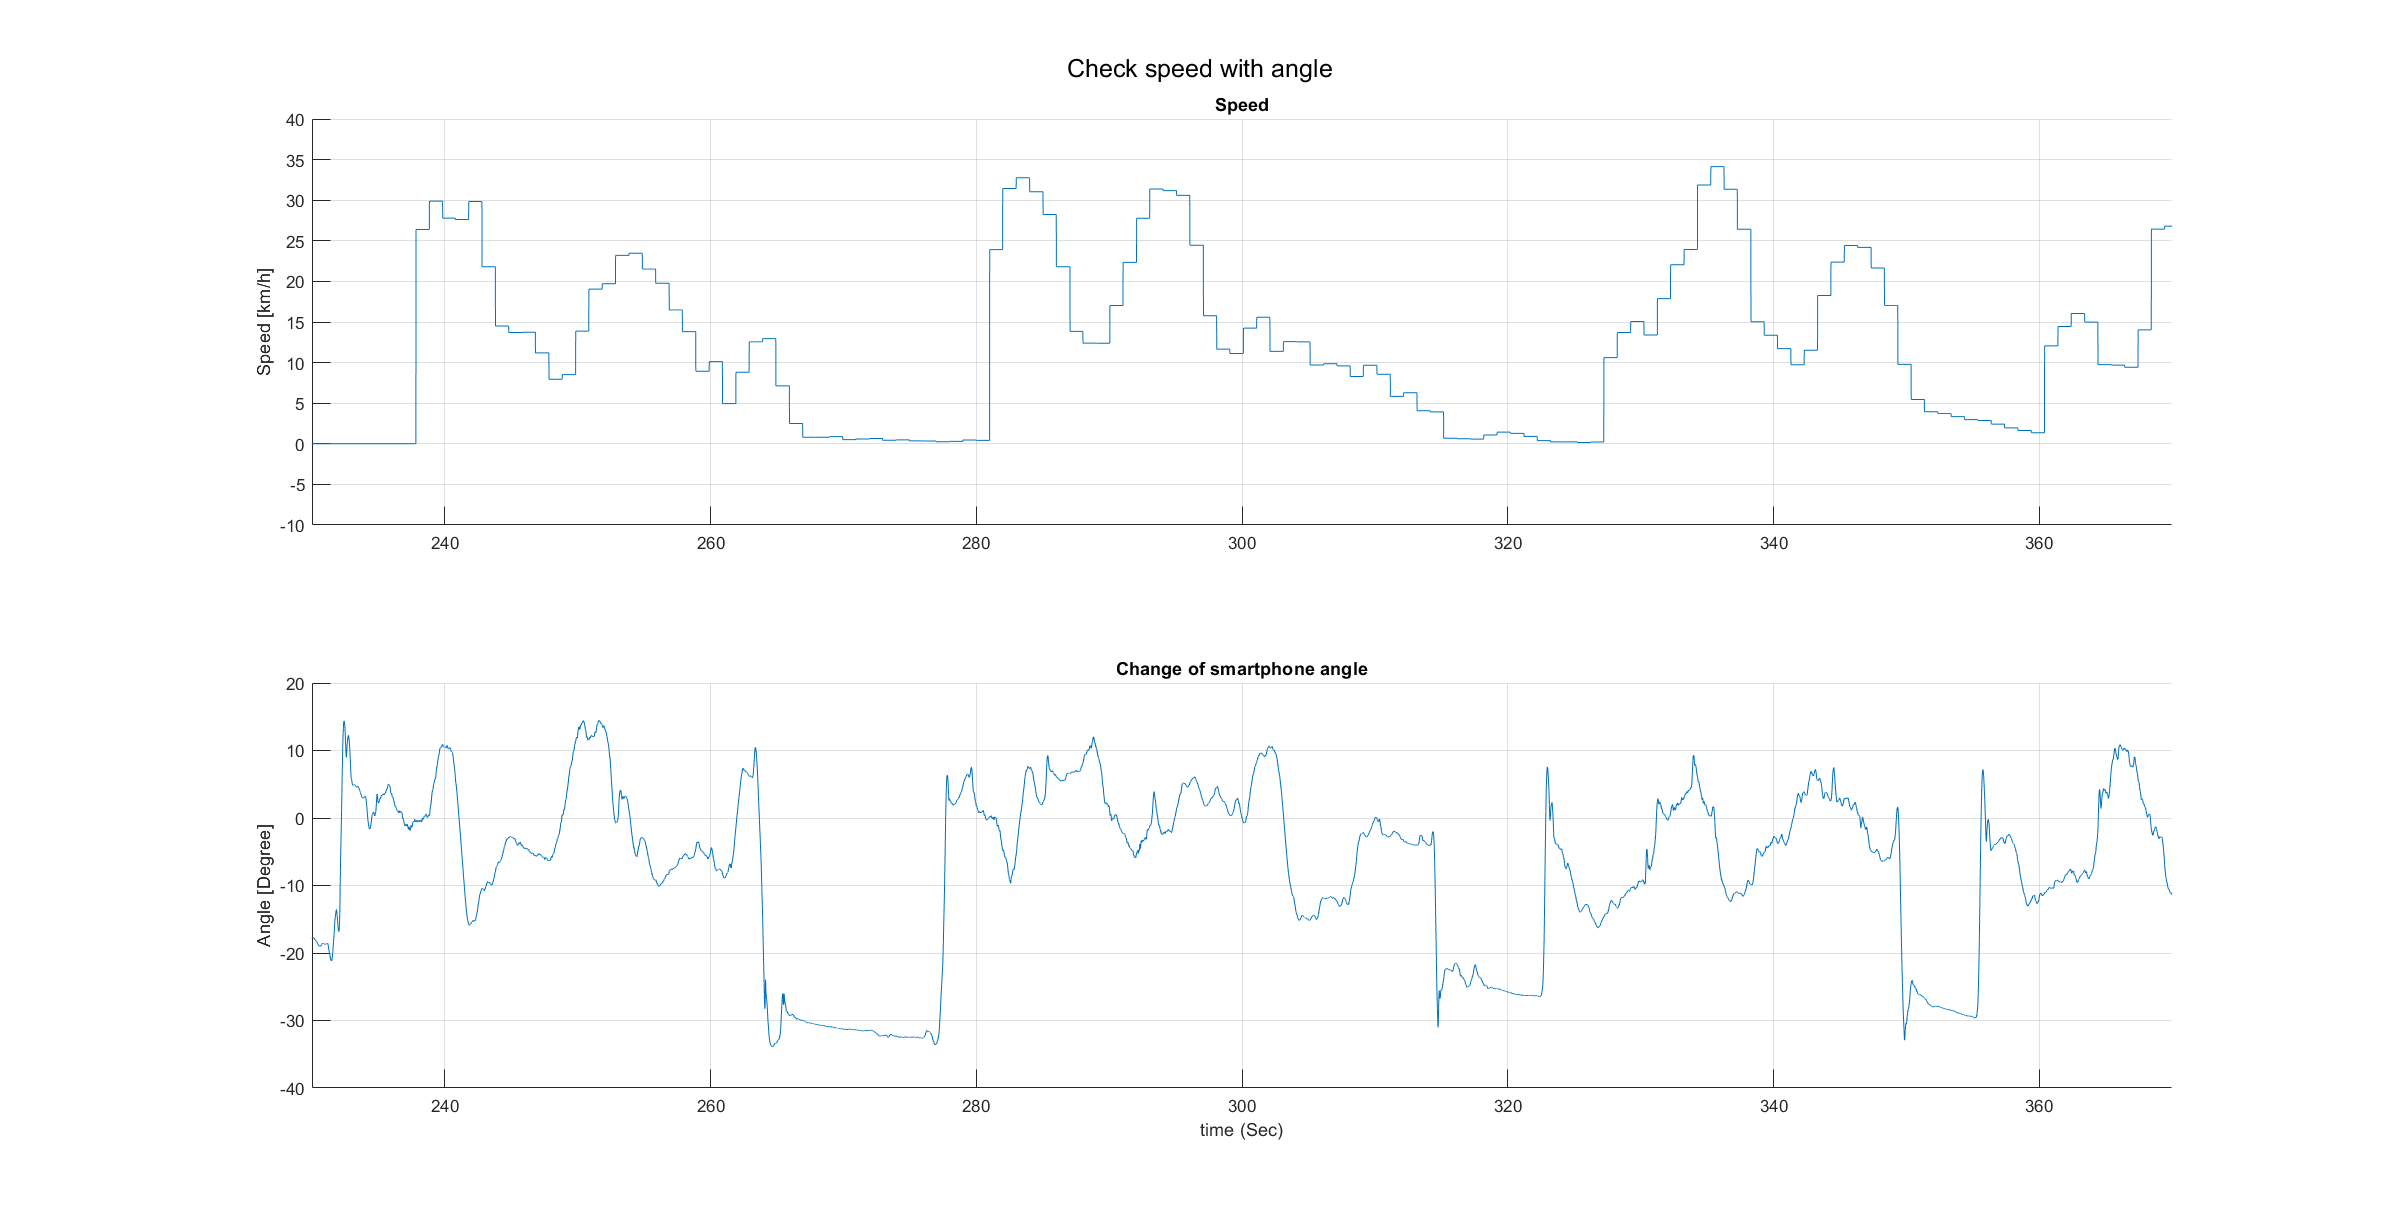
\includegraphics[width=\linewidth]{Bilder/Speed_AngleChangeCompare.png}
	\caption{Winkeländerung des Smartphones durch das Anhalten}
	\label{fig:Speed_AngleChangeCompare}
\end{figure}
Winkeländerung nicht über \ang{45} beträgt $->$ kein Fehlalarm.\\
\\
Beurteilung:

Zu diesem Zweck wurden mehreren Tests durchgeführt, während Diesen keine falsche Alarmauslösungen aktiviert wurden. Grund ist, dass die Winkeländerung nicht \ang{90} beträgt sondern nur ca. \ang{20}-\ang{30} (\autoref{fig:MotorbikeDrivingStanding}). Die Person hat sein Bein beim Sitzen nicht genau horizontal sondern leicht nach Unten geneigt. Und wenn der Fahrer sein Fuß runter setzt, ist diese auch nicht genau vertikal sondern bisschen gebogen mit einem Winkel von ca. \ang{10}-\ang{20} zum Vertikallinie. D.h. die Winkeländerung ist nicht über \ang{45} und sollte zu keinen Alarmauslösungen führen..

\begin{figure}[H]
	\centering
	\begin{subfigure}{\textwidth}
		\centering
		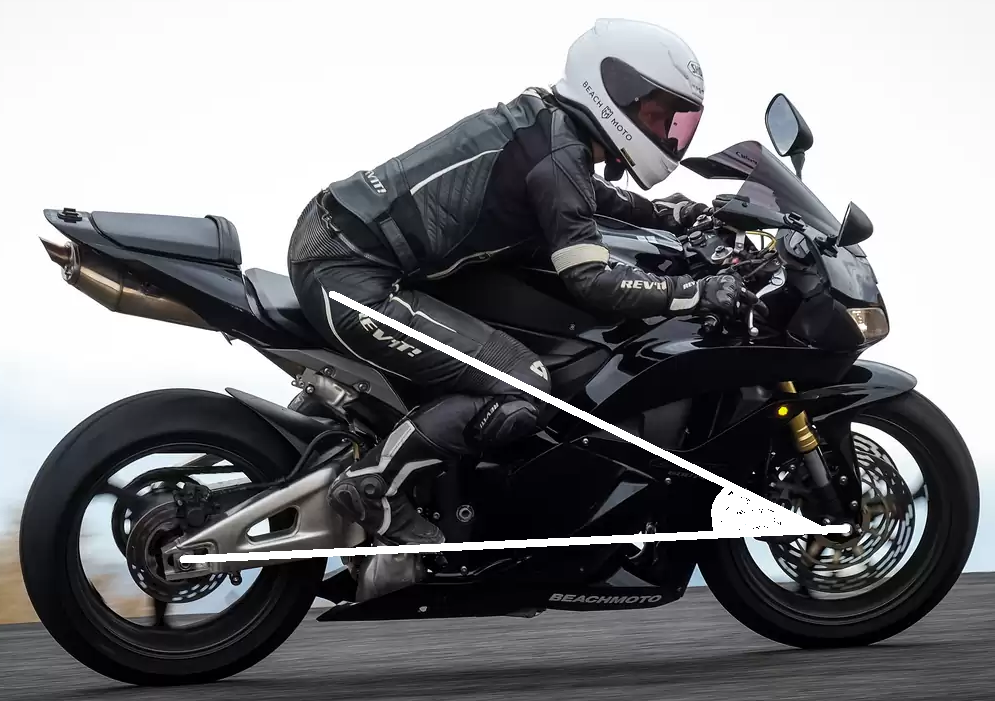
\includegraphics[width=0.5\textwidth]{Bilder/MotorbikeDriving2.png}
		\caption{Beinposition während einer Fahrt}
		\label{fig:MotorbikeDriving}
	\end{subfigure}
	\hfill
	\begin{subfigure}{\textwidth}
		\centering
		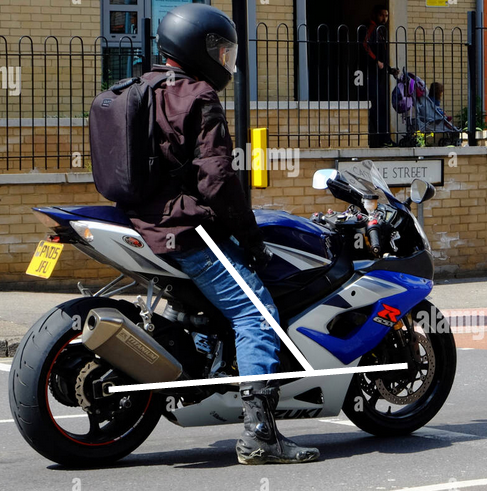
\includegraphics[width=0.5\textwidth]{Bilder/MotorbikeStanding2.png}
		\caption{Beinposition Beim Stehen}
		\label{fig:MotorbikeStanding2}
	\end{subfigure}
	\caption{Beinpositionen während einer Fahrt und gestreckt}
	\label{fig:MotorbikeDrivingStanding}
\end{figure}


\section{Vor- und Nachteile}
- Rechenzeit: kein wesentlicher Unterschied (55 Sec und 57 Sec)





 